\documentclass[13pt,compress]{beamer}

\usepackage{../../summer24/lecture_i2dl/style/lmu-lecture}

\setbeamertemplate{frametitle}{\expandafter\uppercase\expandafter\insertframetitle}
% remove section slides
\AtBeginSection[]
{
  \begin{frame}[plain]
    \frametitle{Introduction to Deep Learning}
	\footnotesize
    \tableofcontents[currentsection]
  \end{frame}
}
\AtBeginSubsection[]
{
  \begin{frame}<beamer>
    \frametitle{}
\begin{center}    
\Large{\subsecname}
\end{center}
  \end{frame}
}
% includepdf slides, pagecommad will set counter for framenumber
\usepackage{pdfpages}
\includepdfset{trim=0mm 0mm 0mm 0mm, pagecommand={\global\setcounter{framenumber}{\value{page}}}}
% add footer:
\usepackage{framed, color}
\usepackage{xcolor}
\setbeamertemplate{footline}[text line]{%
    \noindent\hspace*{\dimexpr-\oddsidemargin-1in\relax}%
     \colorbox{white}{
     \makebox[\dimexpr\paperwidth-2\fboxsep\relax]{
     \color{black}
     \begin{minipage}[c][4.5ex][c]{0.7\linewidth}
       \secname \, | \subsecname
     \end{minipage}
     \hfill\begin{minipage}[c][4.5ex][c]{0.3\linewidth}
       \flushright
       \insertframenumber{}~/~\inserttotalframenumber~~
     \end{minipage}
     }}%
  \hspace*{-\paperwidth}
}

\title{Introduction to Deep Learning}
\author{Prof.~Dr.~David R\"ugamer}
\institute{LMU Munich, MCML}
\date{2023}

\begin{document}
\setbeamercolor{background canvas}{bg=}

% General remark: hyperlinks in included pdfs are not clickable anymore in the combined pdf


\begin{frame}[plain]
  \titlepage
\end{frame}
\begin{frame}[plain]{Introduction to Deep Learning}
\tableofcontents[sectionstyle=show/show, subsectionstyle=hide/hide]
\end{frame}
\section{Introduction \& MLPs}
\subsection{Introduction}
\includepdf[pages={2-7}]{../../summer24/lecture_i2dl/slides-pdf/topic1/slides-intro-introduction.pdf}
\subsection {A Single Neuron}
\includepdf[pages={2-10}]{../../summer24/lecture_i2dl/slides-pdf/topic1/slides-mlps-single-neuron.pdf}
\subsection{Single Hidden Layer Networks}
\includepdf[pages={3-last}]{../../summer24/lecture_i2dl/slides-pdf/topic1/slides-mlps-single-hidden-layer-networks.pdf}
\subsection{Multiclass Classification}
\includepdf[pages={2-5}]{../../summer24/lecture_i2dl/slides-pdf/topic1/slides-mlps-multiclass-classification.pdf}
\subsection{Multilayer MLPs}
\includepdf[pages={2-4, 17}]{../../summer24/lecture_i2dl/slides-pdf/topic1/slides-mlps-multilayer-FNNs.pdf}
\subsection{Basic Training}
\includepdf[pages={2}]{../../summer24/lecture_i2dl/slides-pdf/topic2/slides-opt1-basic-training.pdf}
\includepdf[pages={14}]{../../summer24/lecture_i2dl/slides-pdf/topic1/slides-mlps-multiclass-classification.pdf}
\includepdf[pages={3-4}]{../../summer24/lecture_i2dl/slides-pdf/topic2/slides-opt1-basic-training.pdf}
\includepdf[pages={19-20}]{../../summer24/lecture_i2dl/slides-pdf/topic4/slides-optim-challenges.pdf}
\includepdf[pages={6-last}]{../../summer24/lecture_i2dl/slides-pdf/topic2/slides-opt1-basic-training.pdf}
\section{Convolutional Neural Networks}
\subsection{Introduction}
\includepdf[pages={2-last}]{../../summer24/lecture_i2dl/slides-pdf/topic5/slides-cnn-introduction.pdf}
\subsection{Conv2D}
\includepdf[pages={2-16}]{../../summer24/lecture_i2dl/slides-pdf/topic5/slides-cnn-conv2d.pdf}
\subsection{Properties of Convolutional Layers}
\includepdf[pages={2-last}]{../../summer24/lecture_i2dl/slides-pdf/topic5/slides-cnn-properties-of-convolution.pdf}
\subsection{Components of Convolution Layers}
\includepdf[pages={4-10,13-15, 17-19}]{../../summer24/lecture_i2dl/slides-pdf/topic5/slides-cnn-components.pdf}
\section{Recurrent Neural Networks}
\subsection{Introduction}
\includepdf[pages={3}]{../../summer24/lecture_i2dl/slides-pdf/topic7/slides-introduction.pdf}
\includepdf[pages={20-21,25-26}]{../../summer24/lecture_i2dl/slides-pdf/topic8/slides-applications.pdf}
\includepdf[pages={4-9,11-17}]{../../summer24/lecture_i2dl/slides-pdf/topic7/slides-introduction.pdf}
\subsection{Modern RNNs}
\includepdf[pages={3-13,15-21,23-24}]{../../summer24/lecture_i2dl/slides-pdf/topic7/slides-modernrnn.pdf}
\subsection{Encoder-Decoder Networks and Attention}
\includepdf[pages={15-18}]{../../summer24/lecture_i2dl/slides-pdf/topic8/slides-applications.pdf}
\includepdf[pages={3-6,10-12}]{../../summer24/lecture_i2dl/slides-pdf/topic8/slides-attention.pdf}
\section{Practical Considerations for Training Neural Networks}
\subsection{Hardware and Software}
\includepdf[pages={3-5,9-10}]{../../summer24/lecture_i2dl/slides-pdf/topic2/slides-opt1-hardware-and-software.pdf}
\subsection{Regularization}
\includepdf[pages={6, 11-14, 19-21}]{../../summer24/lecture_i2dl/slides-pdf/topic3/slides-regu-ensemble-dropout-augmentation.pdf}
\subsection{Advanced Training}
\includepdf[pages={3-4,8-9,18-23,25-31,36-41}]{../../summer24/lecture_i2dl/slides-pdf/topic4/slides-advanced-optim.pdf}
\subsection{Activation Functions}
\includepdf[pages={3-10}]{../../summer24/lecture_i2dl/slides-pdf/topic4/slides-activations.pdf}
\subsection{Residual Connections}
\includepdf[pages={7-14}]{../../summer24/lecture_i2dl/slides-pdf/topic6/slides-modern-cnn-2.pdf}
\section*{Outlook}
\subsection*{Autoencoders}
\begin{frame}<beamer>[plain]
    \frametitle{}
\begin{center}    
\Large{Outlook: Autoencoders}
\end{center}
  \end{frame}
\includepdf[pages={2,7-10}]{../../summer24/lecture_i2dl/slides-pdf/topic9/slides-autoencoders.pdf}
\begin{frame}<beamer>[plain]
    \frametitle{}
\begin{center}    
\Large{Outlook: Generative  Adversarial Networks}
\end{center}
  \end{frame}
\subsection*{Generative Adversarial Networks}
\includepdf[pages={2,3}]{../../summer24/lecture_i2dl/slides-pdf/topic10/slides-gan.pdf}
\begin{frame}<beamer>[plain]
    \frametitle{}
\begin{center}    
\Large{Outlook: Overview Generative Models}
\end{center}
  \end{frame}
\subsection*{Overview Generative Models}
\begin{frame}
    \frametitle{Overview Generative Models}
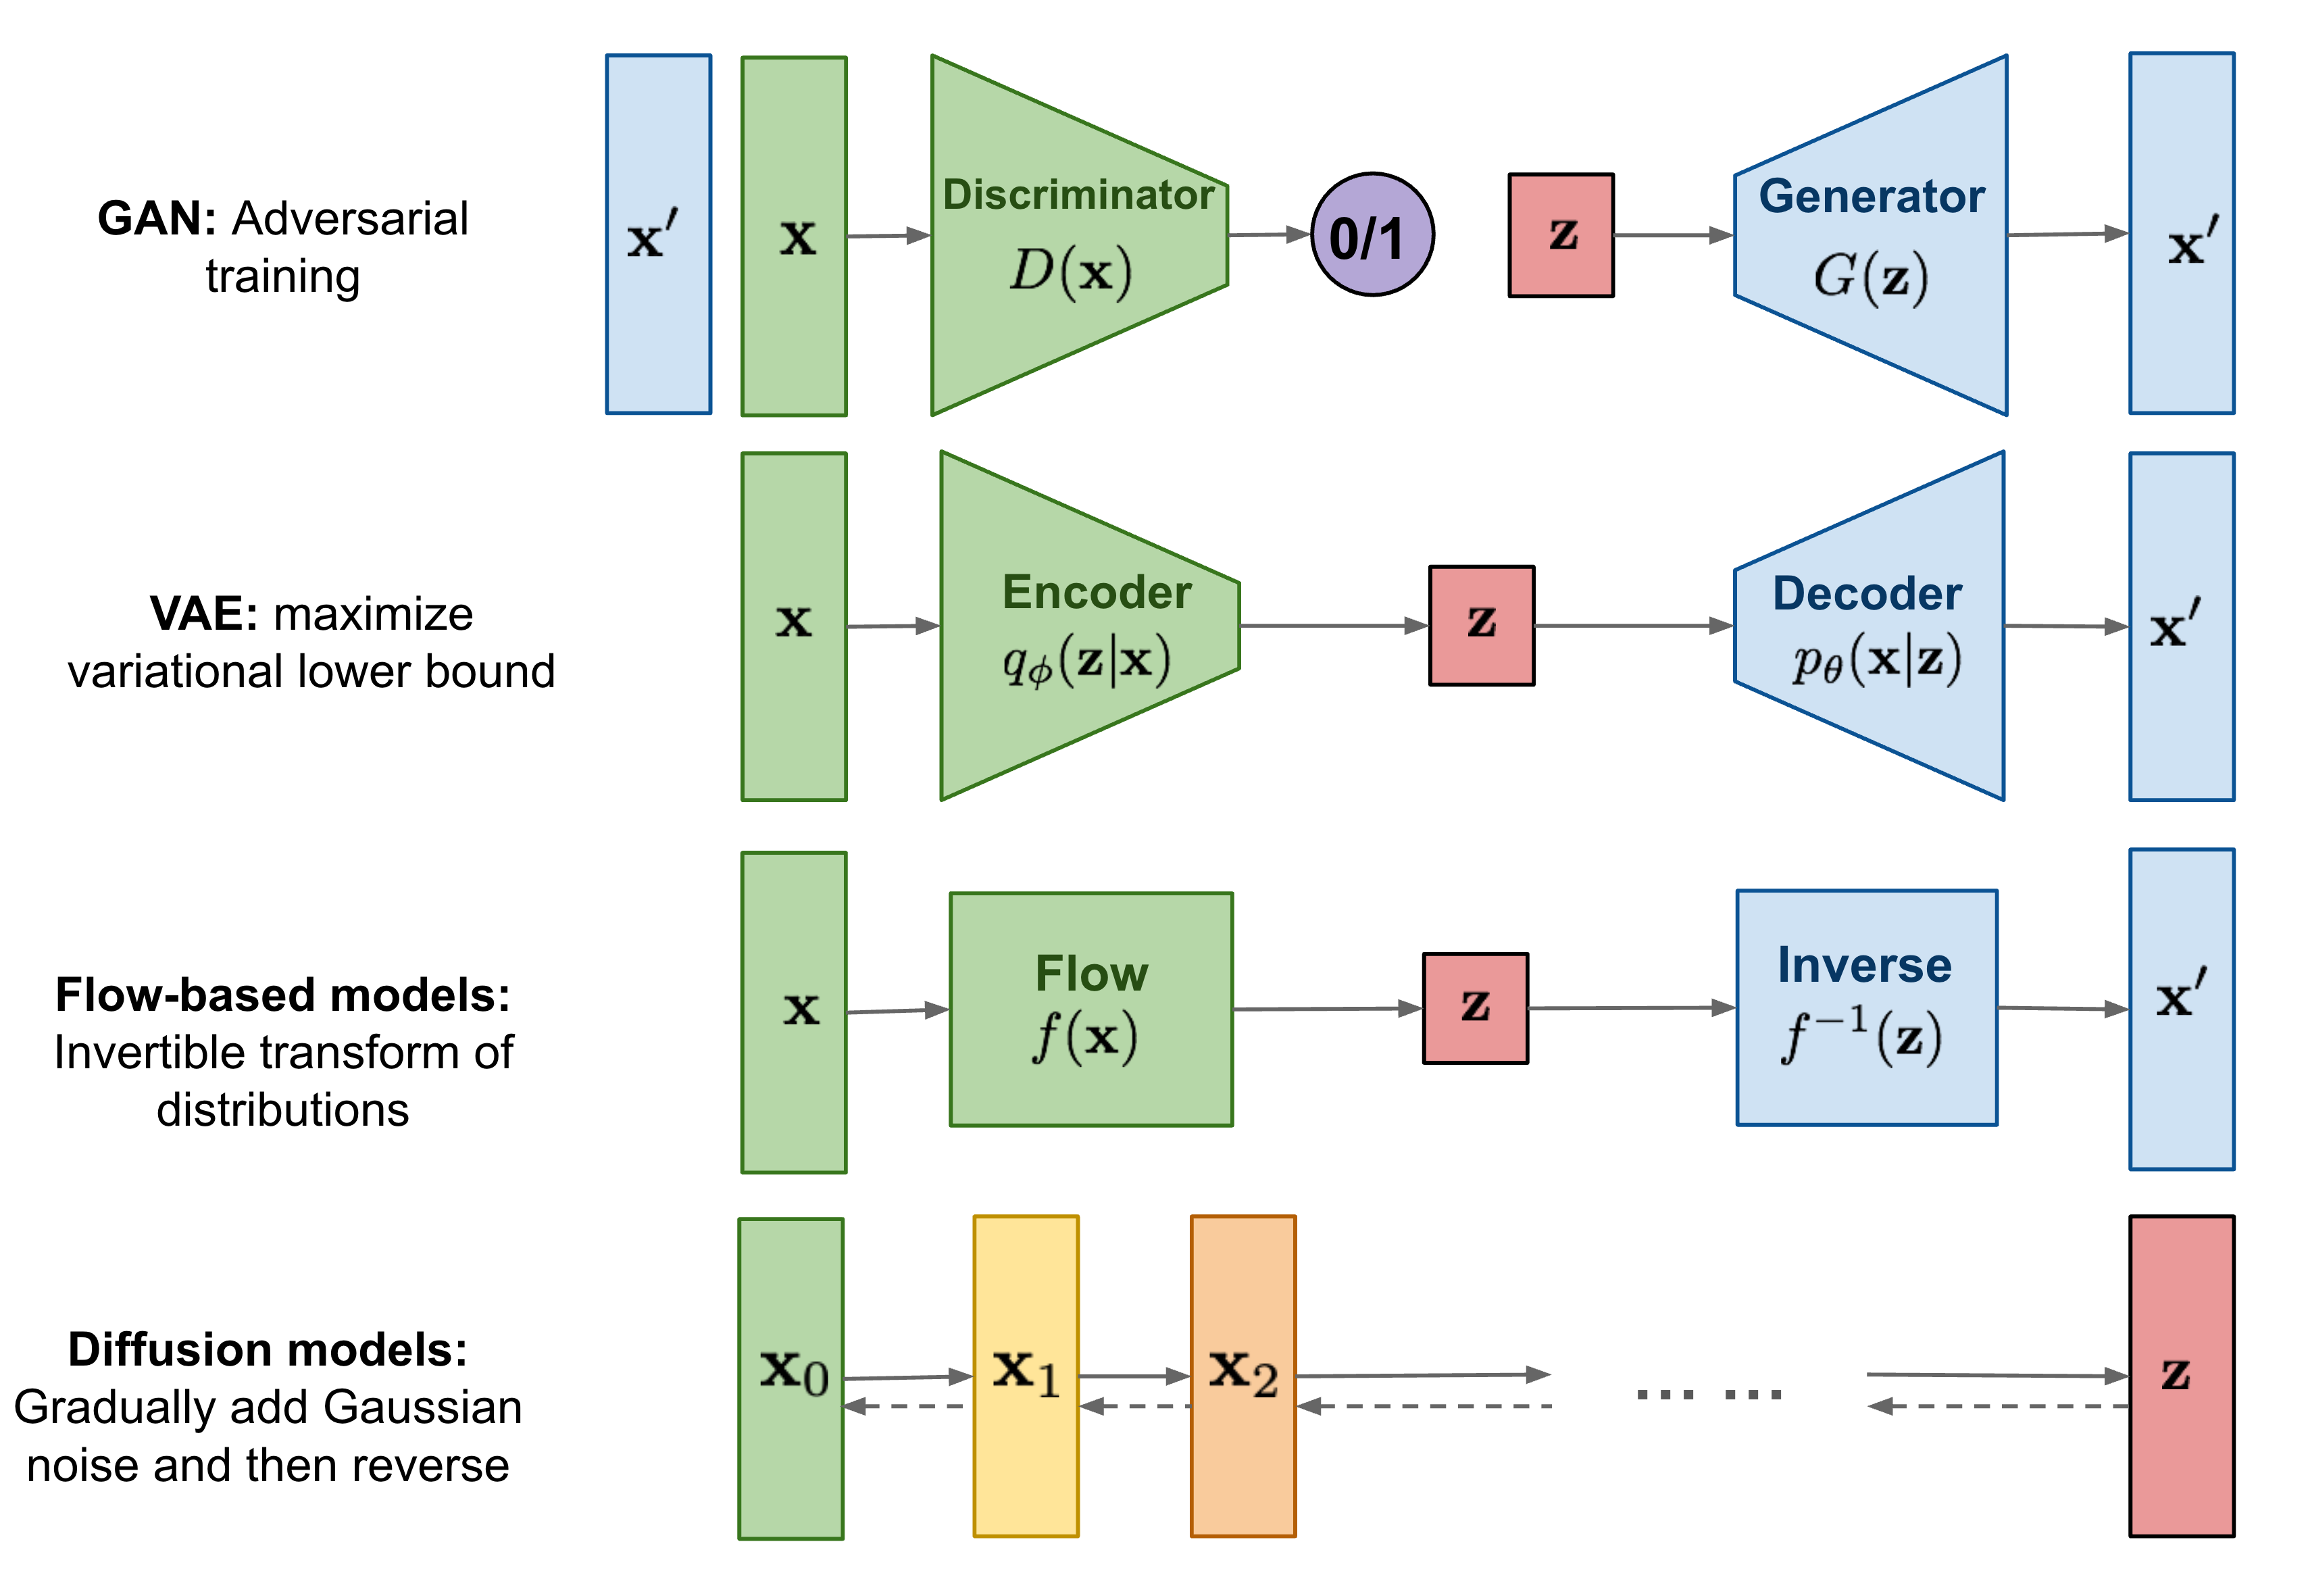
\includegraphics[width=\textwidth]{generative-overview.png}\\
\hfill \begin{tiny}
Source: lilianweng.github.io
\end{tiny}
  \end{frame}
\end{document}
